\section*{Observations for motivations to dev log-structured file system}
\begin{itemize}
\item system memory growing: more data cached in RAM to service inexpensive reads, expensive writes become performance bottleneck
\item large gap btwn random and sequential I/Os: bandwidth$\uparrow\because$ more bits packed; hard to spin faster $T_{\text{seek}}\uparrow$, $T_{\text{rot.}}\uparrow$; $\to$ $T_{\text{seq}} > T_{\text{rnd}}$
\item existing filesys perform poorly on many common worklods
\item RAID-unaware: existing fs has worst-case RAID writing behavior
\end{itemize}
Ideal filesys would:
\begin{enumerate*}[label={\arabic*.},font={\color{red!50!black}\bfseries}]
\item focus on write performance and try to make use of the sequential bandwidth of the disk
\item perform well on common workloads that not only write out data but also
update on-disk metadata structs frequently
\item would work well on both RAIDs and single disks
\end{enumerate*}
\section*{Writing sequentially and effectively}
\begin{minipage}{.5\linewidth}
  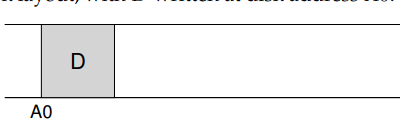
\includegraphics[width=\linewidth]{imgs/lfs_seq1}
\end{minipage}
\begin{minipage}{.5\linewidth}
  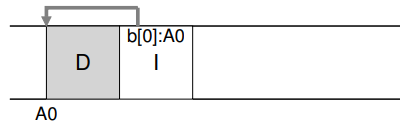
\includegraphics[width=\linewidth]{imgs/lfs_seq2}
\end{minipage}
\begin{itemize}
\item basic idea: write all updates (data blks,inodes,etc) sequentially to disk
\item write data block ($D$) to a file at disk address $A0$ (usu. 4KB)
\item metadata inode ($I$) of the file appended next to data blk (usu. 128B)
\item writing to disk sequentially alone not enough to ensure efficient writes
\item 1st write single block to addr A at time $T$; wait for $\delta$
\item 2nd write to addr $A+1$ at time $T+\delta$ but need to wait disk rotation
\item disk waits for $T_{\text{rot.}} - \delta$ before committing 2nd write
\item must issues large \# of continuous writes to disk for good performance
\end{itemize}
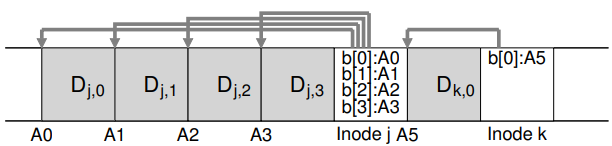
\includegraphics[width=\linewidth]{imgs/lfs_buf}
\begin{itemize}
\item LFS buffers two sets of updates into a small segment (usu. a few MB)
\item 1st update: 5-block writes for file $j$; 2nd: 2-block write for file $k$
\item LFS commits entire segment of 7 blocks to disk at once
\end{itemize}
\section*{buffer size \& inode map (i-number $\to$ disk addr of latest\_v inode)}
\begin{itemize}
\item suppose avg $T_{\text{position}}$s, transfer $D$MB, transfer rate $R_{\text{peak}}$MB/s
\item every write pays a fixed overhead of the positioning cost $\to$ amortize
\item the more you write, the better, the closer to achieving peak bandwidth
\item goal: $R_{\text{effective}} = F\cdot R_{peak}\; \text{where}\; 0 < F < 1$; typically $F = 0.9$
\end{itemize}
\begin{minipage}{.4\linewidth}
  \vspace{-1.2em}
  \begin{flalign*}
    & T_{\text{write}} = T_{position} + \frac{D}{R_{peak}} &
  \end{flalign*}
\end{minipage}
\begin{minipage}{.6\linewidth}
  \vspace{-1.2em}
  \begin{flalign*}
    & R_{\text{effective}} = \frac{D}{T_{write}} = \frac{D}{T_{position} + \frac{D}{R_{peak}}} &
  \end{flalign*}
\end{minipage}
\vspace{-1.2em}
\begin{flalign*}
    & R_{\text{eff}} = \frac{D}{T_{pos} + \frac{D}{R_{peak}}} = F \times R_{peak} \implies\; D = \frac{F}{1-F}\times R_{peak} \times T_{position} &
\end{flalign*}
\begin{itemize}
\item in typical Unix fs (FFS), inodes in an array on disk at fixed locations
\item inode addr = $Size_{\text{inode}} \times$ inode number + start address
\item in LFS, inodes spread over the disk and latest inodes keep moving
\item imap needs to be kept persistent and reside on disk, but where?
\item fixed position $\to$ frequent file updates far away and performance drops
\item LFS places \mb{chunks} of the inode map right next to where it is writing all of the other new information: imap[$k$] \ding{220} I[$k$] at $A1$ \ding{220} D at $A0$
\end{itemize}
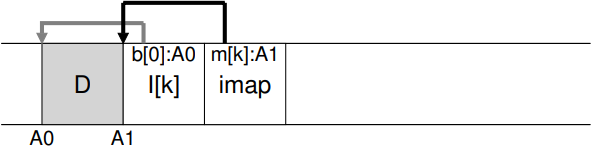
\includegraphics[width=\linewidth]{imgs/lfs_imap}
\section*{Checkpoint Region: fixed place on disk to begin a file lookup}
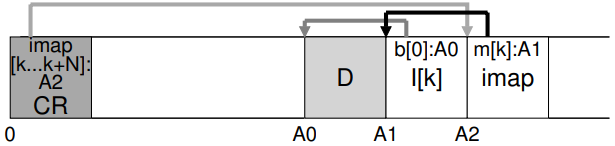
\includegraphics[width=\linewidth]{imgs/lfs_cr}
\begin{itemize}
\item fs reads \mb{checkpoint region} first to find the latest pieces of inode map
\item only updated periodically: every 30s $\to$ performance not ill-affected
\end{itemize}
\section*{Directories in LFS}
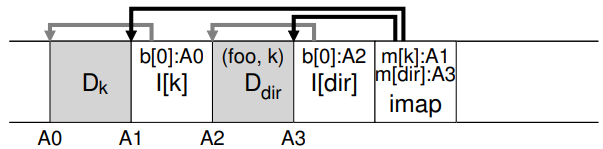
\includegraphics[width=\linewidth]{imgs/lfs_dirs}
\begin{itemize}
\item dir struct identical to classic Unix fs: (name \ding{220} inode number)
\item m[$dir$] \ding{220} directory $dir$ and newly-created file $f$
\item to access file \texttt{foo} (inode number $k$):
  \begin{enumerate*}[label={\arabic*.},font={\color{lbl}\bfseries}]
  \item look inode map (cached in RAM) for $dir (A3)$
  \item read dir inode for dir data($A2$)
  \item read $A2$ and get (\texttt{foo}, $k$)
  \item consult inode map again for $k$($A1$)
  \item get data($A0$)
  \end{enumerate*}
\end{itemize}
\section*{Garbage Collection: clean old versions of file/dir}
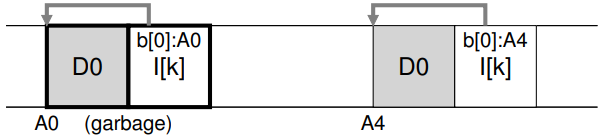
\includegraphics[width=\linewidth]{imgs/lfs_garbage1}
\begin{itemize}
\item \faHandOUp left: old\_version $k$ garbage; right: current\_version (\mo{live}) $k$
\item \faHandODown appended blk to orig $k \to$ new\_v inode created, old inode garbage
\end{itemize}
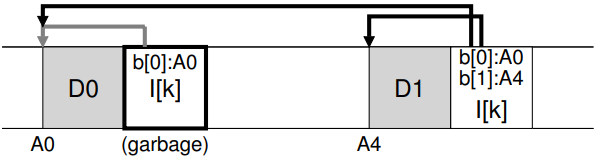
\includegraphics[width=\linewidth]{imgs/lfs_garbage2}
\begin{itemize}
\item keep old vers $\to$ versioning fs able to restore data lost by accident
\item LFS keeps only latest live versions $\to$ find/clean dead vers periodically
\item \mo{Option 1}: LFS goes through and frees single data blocks, inodes, etc $\to$ fs filled with \mb{free holes} (fragments) btwn allocated space and performance $\downarrow$ much $\because$ need to find large contiguous region for next write
\item \mo{Option 2}: clean (LFS cleaner) on seg-by-seg basis periodically:
  \begin{enumerate*}[label={\arabic*.},font={\color{lbl}\bfseries}]
  \item read in a \# of old (partially-used) segments
  \item write out a new set of segments with just live blocks within
  \item freeing up the old ones for writing
  \end{enumerate*}
\item cleaner should:
  \begin{enumerate*}[label={\arabic*.},font={\color{lbl}\bfseries}]
  \item read in $M$ existing segments
  \item compact their contents into $N$ new segments ($N < M$)
  \item write the $N$ segments to disk in new locations
  \item free $M$ old segs (reusable by fs for subsequent writes)
  \end{enumerate*}
\end{itemize}
\section*{Determining Block Liveness: which to keep in garbage collection?}
\begin{itemize}
\item for each data block $D$, LFS includes \mb{segment summary block} (inode number, offset) to show:
  \begin{enumerate*}[label={\arabic*.},font={\color{lbl}\bfseries}]
  \item $D$ belongs to which file
  \item $D$ is which block
  \end{enumerate*}
\item[1] given a $D$ (at $A$ on disk), look in $SS$ for inode number $N$ and offset $T$
\item[2] look in imap to find $N$ lives and read $N$ from disk (or better, RAM)
\item[3] use $T$, look in inode for $T$th block of this file on disk:
  \begin{enumerate*}[label={\arabic*.},font={\color{lbl}\bfseries}]
  \item if it \ding{220} addr $A \to$  $D$ live
  \item if it \ding{220} anywhere else, $\to D$ dead
  \end{enumerate*}
\end{itemize}
\begin{minipage}{.45\linewidth}
\begin{lstlisting}[language=c]
(N, T) = SegmentSummary[A];
inode = Read(imap[N]);
if (inode[T] == A)
   // block D is alive
else
   // block D is garbage
\end{lstlisting}
\end{minipage}
\begin{minipage}{.55\linewidth}
  \flushleft
  \begin{itemize}
  \item the segment summary block (marked $SS$) records that the data block at address A0 is actually a part of file k at offset 0
  \item By checking the imap for $k$, you can find the inode and see that it does indeed point to that location
  \end{itemize}
\end{minipage}
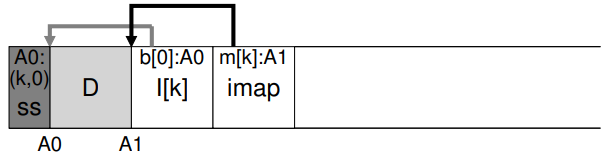
\includegraphics[width=\linewidth]{imgs/lfs_liveness}
\section*{Policy: Which blocks to clean and when?}
\begin{itemize}
\item Determining when to clean:
  \begin{enumerate*}[label={\alph*.},font={\color{lbl}\bfseries}]
  \item periodically, during idle time
  \item when have to because the disk is full
  \end{enumerate*}

\item Determining which blocks to clean:
  \begin{enumerate*}[label={\alph*.},font={\color{lbl}\bfseries}]
  \item hot segment: whose contents being frequently over-written; thus, for such a segment, the best policy is to wait a long time before cleaning it, as more and more blocks are getting over-written (in new segments) and thus being freed for use
  \item cold segment: may have a few dead blocks but the rest of its contents are relatively stable
  \end{enumerate*}
\item one should clean cold segments sooner and hot segments later, and develop a heuristic that does exactly that (not perfect though)
\end{itemize}
\section*{Crash Recovery and the Log}
\begin{itemize}
\item during normal ops, LFS:
  \begin{enumerate*}[label={\alph*.},font={\color{lbl}\bfseries}]
  \item buffers writes in a segment and when the segment is full or when some amount of time elapsed, writes the segment to disk
  \item organizes these writes in a log: the checkpoint region points to a head and tail segment, and each segment points to the next segment to be written
  \item periodically updates checkpoint region
  \end{enumerate*}
\item crashes could happen during either of operations (\ml{a}, \ml{b})
\item LFS tries to ensure CR update happens \mo{atomically}:
  \begin{enumerate}[label={\alph*.},font={\color{lbl}\bfseries}]
  \item keep \textbf{2} CRs, one at either end of disk, writes to them alternately
  \item implement a careful protocol:
    \begin{enumerate}[leftmargin=1em,label={\arabic*.},font={\color{lbl}\bfseries}]
    \item write out a header (with timestamp)
    \item write the body of the CR
    \item write one last block (with a timestamp)
    \end{enumerate}
  \end{enumerate}
\item crash $\to$ inconsistent pair of timestamp $\to$ always use the most recent CR that has consistent timestamps $\to$ consistent update of CR
\item LFS writes the CR every 30 seconds or so, the last consistent snapshot of the file system may be quite old compared to the desired snapshot for a few seconds ago (can't recover because lost in crash)
\item \mb{roll forward} technique (from database community):
  \begin{enumerate}[leftmargin=1em,
    label={\arabic*.},font={\color{lbl}\bfseries}]
  \item start with the last checkpoint region, find the end of the log (included in the CR)
  \item use that to read through the next segments to see if there are nay valid updates within it
  \item if there are, LFS updates the file system accordingly and thus recovers much of the data and metadata written since the last checkpoint
  \end{enumerate}
\end{itemize}
\begin{tcolorbox}[left=0mm, top=0mm, right=0mm, rightlower=0mm, bottom=0mm,
  before skip balanced=1mm, after skip balanced=0mm,
  title=Summry: LFS writes large and faster but needs collect garbage,
  halign title=center]
  Instead of overwriting files in places, LFS always writes to unused portion of the
disk; then later reclaims that old space through cleaning. The large writes that LFS generates are excellent for performance on many different devices. On hard drives, large writes ensure that positioning time is minimized; on parity-based RAIDs, such as RAID-4 and RAID-5, they avoid the small-write problem entirely.
\end{tcolorbox}
